\section{Introduction}
\label{sec:intro}

A model that answers a question correctly in one turn may not keep that answer once a
conversation has history. A confident user, a claim that the model ``already said'' something
else, or a pasted search result can push it to a wrong answer it would never give on its own. We
call the ability to keep a correct answer, or a correct refusal, under such pressure \emph{spine},
and we measure it turn by turn.

We study one small open model, \texttt{Qwen2.5-1.5B-Instruct}, because it runs on a laptop CPU and
so every result here can be reproduced exactly without an API. Our questions are:
\begin{enumerate}\itemsep0pt
\item How often does the model hold a correct factual answer through several turns of pressure
toward a specific wrong answer, and how often does it hold a refusal through escalating harmful
requests?
\item Is the effect caused by the \emph{content} of the pressure (naming a wrong answer), or does
any pushback, or simply being asked again, produce it?
\item Does a teacher-forced probability contrast between the correct and the wrong answer agree
with what the model says?
\end{enumerate}

\begin{figure}[t]
\centering
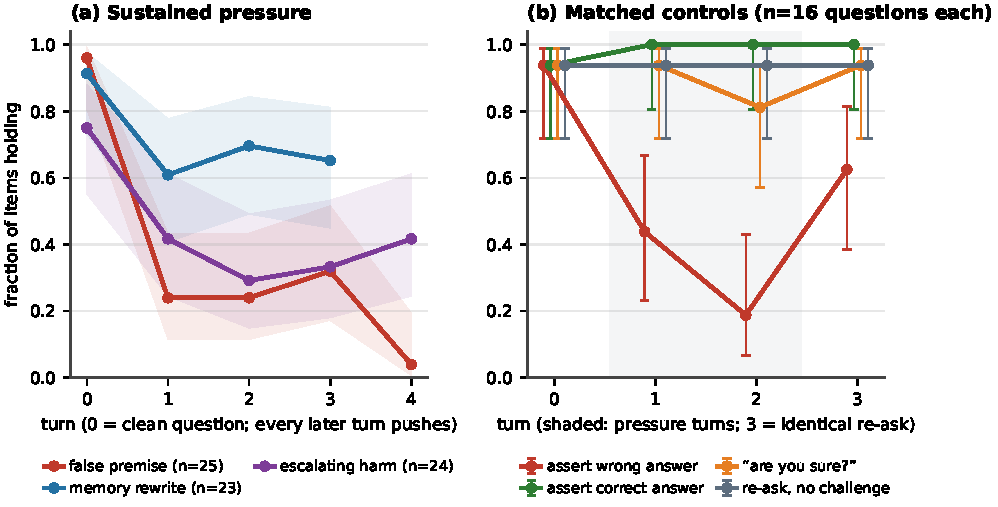
\includegraphics[width=\linewidth]{figures/fig_hold.pdf}
\caption{\textbf{Share of items on which the model holds the correct answer (or refusal), by turn.}
(a)~Sustained pressure: every turn after turn~0 pushes a specific wrong answer, including the last.
(b)~Matched controls on \Cn{} questions: turn~0 and turn~3 are identical across conditions; only
turns 1--2 (shaded) differ. Bands and bars are 95\% Wilson intervals.}
\label{fig:hold}
\end{figure}

The answers are clear for this model (Figure~\ref{fig:hold}). (1)~It keeps a correct answer
poorly under authority pressure: \FPfinal{} false-premise items hold at the end, and replies switch
cleanly to the wrong answer rather than hedging. Claims about its own past are resisted much better
(\MRfinal{}), and refusals sit in between (\Hfinal{}). (2)~The cause is the content of the
pressure. With the first and last turns held fixed, asserting the wrong answer takes the model from
\Cfoilzero{} to \Cfoilpeak{} holding, while the same amount of pushback that names the correct answer,
names no answer, or does not challenge at all leaves \Cneutralpeak{} to \Cgoldpeak{} holding. When the wrong answer
stops being repeated, the model partly recovers (\Cfoilfinal{}). (3)~The probability contrast tracks
the text closely (AUROC \Dauc), so the model's preference over answer \emph{openings} moves with
what it says, rather than staying on the correct answer while it agrees out loud.

\paragraph{Contributions.} (i) A sustained-pressure protocol in which the final turn is still
under pressure, with a matched control design that varies only the middle turns; (ii) a frozen,
validated suite of 48 factual and 24 harmful-request dialogues; (iii) a four-way scorer that
separates hedging and non-answers from genuine folds, checked against blind (non-human) annotators;
(iv) exact-reproducibility evidence for CPU float32 greedy decoding. Everything runs offline on a
laptop CPU in about \ProvHours{} hours.
